\subsection{SensTool}
A lot of the background for the implementation above comes from documentation on a Matlab toolbox called SensTool \fxnote{Reference Senstool guide}. The optimization method is implemented in it and it also includes an extra feature based on parameter sensitivity and frequency domain. For a better accuracy on the estimation it is a good decision to use this tool as the final approach to the parameters of the Cubli model.

The same data, Simulink model and initial parameters as the previous case are given to this toolbox and the result of the fit can be seen in \figref{SenseToolParameterEstimation}. 
%
\begin{figure}[H]
	\centering
	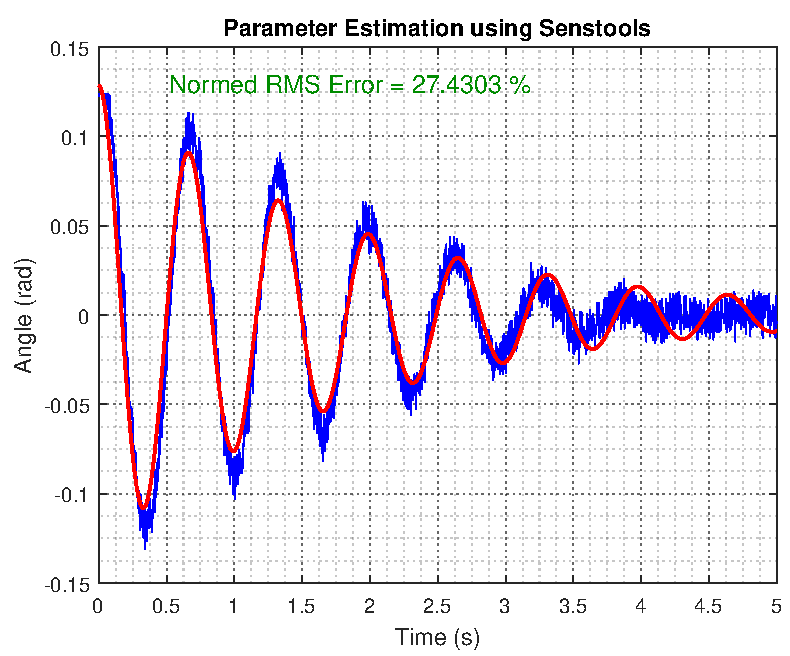
\includegraphics[scale=0.7]{figures/SenseToolParameterEstimation}
	\caption{Data from the test (red) and final fit with the new parameters (blue)}
	\label{SenseToolParameterEstimation}
\end{figure}

The final estimated parameters are \si{J_F=4,8 \cdot 10^{-3}\ kg \cdot m^2\ and\ B_F=7,7 \cdot 10^{-3}\ m \cdot s \cdot rad^{-1}}. The normed RMS error is \si{27,4\ \%} compared to the \si{31,7\ \%} shown in \figref{ParameterEstimationNewtonCubli}. The \si{4,3\ \%} error reduction is likely due to additional algorithms.

\section{Final Parameters}
The final parameters of the system can be seen in \ref{ParametersSystem}
\begin{table}[H]
	\begin{tabular}{|l|l|p{3cm}|}
		\hline %-----------------------------------------------------------------------------------
		\textbf{Parameter} &\textbf{Value} &\textbf{Units}\\
		\hline %-----------------------------------------------------------------------------------
		\si{m_w}         & \si{0,222}       &kg\\
		\hline
		%-----------------------------------------------------------------------------------
		\si{l_w}         & \si{0,096}       &m\\
		\hline %-----------------------------------------------------------------------------------
		\si{J_w}            & \si{0,601 \cdot 10^{-3}}	&\si{kg \cdot m^2}\\
		\hline  
		%-----------------------------------------------------------------------------------
		\si{B_w}         & \si{17,03 \cdot 10^{-6}}       &N \si{\cdot m \cdot s \cdot rad^{-1}}\\
		\hline
		%-----------------------------------------------------------------------------------
		\si{m_F}         & \si{0,548}       &kg\\
		\hline
		%-----------------------------------------------------------------------------------
		\si{l_F}         & \si{0,08498}       &m\\
		\hline %-----------------------------------------------------------------------------------
		\si{J_F}            & \si{4,8 \cdot 10^{-3}}	&\si{kg \cdot m^2}\\
		\hline %-----------------------------------------------------------------------------------
		\si{B_F}         & \si{7,7 \cdot 10^{-3}}       &N \si{\cdot m \cdot s \cdot rad^{-1}}\\
		\hline
	\end{tabular}
	\caption{Parameters of the whole system}
	\label{ParametersSystem}
\end{table}